\documentclass[12pt,a4paper,oneside]{report}

% -----------------------------------------------------------------------------
% PACKAGES & CONFIGURATION
% -----------------------------------------------------------------------------
\usepackage[utf8]{inputenc}
\usepackage[T1]{fontenc}
\usepackage{lmodern}
\usepackage[margin=1in,headheight=15pt]{geometry}
\usepackage{graphicx}
\usepackage{amsmath,amssymb}
\usepackage{booktabs}
\usepackage{tabularx}
\usepackage{longtable}
\usepackage{multirow}
\usepackage{xcolor}
\usepackage{listings}
\usepackage{fancyhdr}
\usepackage{titlesec}
\usepackage{setspace}
\usepackage{enumitem}
\usepackage{tikz}
\usetikzlibrary{shapes.geometric, arrows, positioning, fit, calc}
\usepackage[colorlinks=true, linkcolor=blue!70!black, citecolor=blue!70!black, urlcolor=blue!70!black]{hyperref}

\setstretch{1.2}

% -----------------------------------------------------------------------------
% COLOR PALETTE (Matched to ClinicTrack Brand)
% -----------------------------------------------------------------------------
\definecolor{ctPrimary}{HTML}{0D9488}      % Teal / Primary
\definecolor{ctDark}{HTML}{0F172A}         % Slate Dark
\definecolor{ctAccent}{HTML}{3B82F6}       % Blue Accent
\definecolor{ctBg}{HTML}{F8FAFC}           % Off-white
\definecolor{ctBorder}{HTML}{CBD5E1}       % Slate Light
\definecolor{codeBg}{HTML}{F1F5F9}         % Light gray for listings
\definecolor{codeGreen}{HTML}{16A34A}      % Comments
\definecolor{codePurple}{HTML}{7C3AED}     % Keywords
\definecolor{codeRed}{HTML}{DC2626}        % Strings

% -----------------------------------------------------------------------------
% CODE LISTING STYLE
% -----------------------------------------------------------------------------
\lstdefinestyle{clinictrackCode}{
    backgroundcolor=\color{codeBg},
    basicstyle=\ttfamily\footnotesize,
    breakatwhitespace=false,
    breaklines=true,
    captionpos=b,
    commentstyle=\color{codeGreen}\itshape,
    keywordstyle=\color{codePurple}\bfseries,
    stringstyle=\color{codeRed},
    numberstyle=\tiny\color{gray},
    numbers=left,
    numbersep=8pt,
    showspaces=false,
    showstringspaces=false,
    showtabs=false,
    tabsize=2,
    frame=single,
    rulecolor=\color{ctBorder},
    frameround=tttt
}
\lstset{style=clinictrackCode}

% -----------------------------------------------------------------------------
% HEADERS & FOOTERS
% -----------------------------------------------------------------------------
\pagestyle{fancy}
\fancyhf{}
\fancyhead[L]{\small\textsf{ClinicTrack — Version-Tracked Patient Record System}}
\fancyhead[R]{\small\textsf{Web Technology Mini-Project}}
\fancyfoot[L]{\small\textsf{MIT Academy of Engineering | Batch A2}}
\fancyfoot[R]{\small\thepage}
\renewcommand{\headrulewidth}{0.4pt}
\renewcommand{\footrulewidth}{0.4pt}

% -----------------------------------------------------------------------------
% CHAPTER FORMATTING
% -----------------------------------------------------------------------------
\titleformat{\chapter}[display]
  {\normalfont\huge\bfseries\color{ctDark}}
  {\chaptertitlename\ \thechapter}{15pt}{\Huge\color{ctPrimary}}
\titlespacing*{\chapter}{0pt}{10pt}{20pt}

% -----------------------------------------------------------------------------
% DOCUMENT METADATA
% -----------------------------------------------------------------------------
\newcommand{\projectTitle}{ClinicTrack: A Version-Tracked Patient Record \& Clinical Management System}
\newcommand{\courseName}{Web Technology (Course Code: 2310362L)}
\newcommand{\academicYear}{2025--2026}
\newcommand{\institutionName}{MIT Academy of Engineering, Alandi, Pune}
\newcommand{\departmentName}{School of Computer Engineering and Technology}
\newcommand{\batchGroup}{Batch A2}

\begin{document}

% =============================================================================
% TITLE PAGE
% =============================================================================
\begin{titlepage}
    \centering
    \vspace*{0.5cm}
    
    {\Large\bfseries\color{ctDark} \institutionName \par}
    {\large\color{gray} \departmentName \par}
    \vspace{1.0cm}
    
    \begin{center}
        \rule{0.8\textwidth}{1.5pt} \\[0.4cm]
        {\huge\bfseries\color{ctPrimary} \projectTitle \par}
        \vspace{0.2cm}
        {\large\bfseries A Full-Stack Clinical Web Application with Git-Style EMR Versioning, Live Queue Telemetry \& Cryptographic Audit Chains \par}
        \rule{0.8\textwidth}{1.5pt}
    \end{center}
    
    \vspace{0.8cm}
    {\large\itshape A Mini-Project Report Submitted in Partial Fulfillment of the Requirements for the Course of \par}
    \vspace{0.2cm}
    {\large\bfseries\color{ctDark} \courseName \par}
    {\normalsize Academic Year: \academicYear \par}
    
    \vspace{1.2cm}
    
    \begin{minipage}[t]{0.85\textwidth}
        \begin{center}
        \textbf{\large Submitted By (Group Members - \batchGroup):} \\[0.3cm]
        \begin{tabularx}{\textwidth}{>{\bfseries}l >{\centering\arraybackslash}X r}
            \toprule
            Student Name & PRN & Role / Module Focus \\
            \midrule
            Nupoor Deshpande & 202401100026 & Backend Architecture, Mongo Aggregations \& API \\
            Bhoomi Tiple     & 202401100027 & React Frontend, State, RHF/Yup Validation \\
            Janhavi Hinganghatkar & 202401100025 & Real-Time Socket.IO, SHA-256 Audit \& Public Portal \\
            \bottomrule
        \end{tabularx}
        \end{center}
    \end{minipage}

    \vfill
    
    \begin{minipage}[t]{0.9\textwidth}
        \centering
        \textbf{Project Repository \& Deployment Coordinates:} \\
        \small
        \texttt{Frontend URL (Vercel):} \url{https://clinictrack-client.vercel.app} \\
        \texttt{Backend API (Render):} \url{https://clinictrack-api.onrender.com} \\
        \texttt{Apache Tomcat Portal:} \url{http://localhost:8080/clinictrack/} \\
        \texttt{Source Code Bundle:} \texttt{ClinicTrack-SourceCode.zip} (Submitted on Moodle)
    \end{minipage}

    \vspace{0.5cm}
    {\normalsize\today \par}
\end{titlepage}

% =============================================================================
% CERTIFICATE / EVALUATION SHEET
% =============================================================================
\newpage
\thispagestyle{plain}
\begin{center}
    {\Large\bfseries \institutionName \par}
    {\large \departmentName \par}
    \vspace{0.8cm}
    {\LARGE\bfseries\color{ctDark} CERTIFICATE OF EVALUATION \par}
    \vspace{0.6cm}
\end{center}

This is to certify that the mini-project entitled \textbf{``\projectTitle''} is a bonafide work carried out by the following students of \textbf{\batchGroup} in partial fulfillment of the academic requirements for the course of \textbf{\courseName} during the academic year \textbf{\academicYear}.

\vspace{0.8cm}

\begin{table}[h!]
\centering
\begin{tabularx}{\textwidth}{c l c X}
\toprule
\textbf{Sr. No.} & \textbf{Candidate Name} & \textbf{PRN} & \textbf{Sign / Evaluation Status} \\
\midrule
1. & Nupoor Deshpande & 202401100026 & \rule{3.5cm}{0.4pt} \\
2. & Bhoomi Tiple & 202401100027 & \rule{3.5cm}{0.4pt} \\
3. & Janhavi Hinganghatkar & 202401100025 & \rule{3.5cm}{0.4pt} \\
\bottomrule
\end{tabularx}
\end{table}

\vspace{1.0cm}

The students have individually demonstrated and presented the working project, covering problem formulation, technological stack, major features, database design, two-tier validation, and execution flow to the satisfaction of the examiner.

\vspace{2.5cm}

\noindent
\begin{minipage}[t]{0.45\textwidth}
    \centering
    \rule{5.5cm}{0.4pt} \\
    \textbf{Subject Teacher / Evaluator} \\
    Department of Computer Engineering \\
    MIT Academy of Engineering
\end{minipage}
\hfill
\begin{minipage}[t]{0.45\textwidth}
    \centering
    \rule{5.5cm}{0.4pt} \\
    \textbf{Head of Department} \\
    School of Computer Engg. \& Tech. \\
    MIT Academy of Engineering
\end{minipage}

% =============================================================================
% ABSTRACT
% =============================================================================
\newpage
\thispagestyle{plain}
\begin{center}
    {\Large\bfseries\color{ctDark} ABSTRACT \par}
\end{center}
\vspace{0.5cm}

Traditional Electronic Medical Record (EMR) systems in small-to-midscale outpatient clinics suffer from two critical architectural pitfalls: destructive in-place overwriting of diagnostic notes (leading to loss of clinical context and malpractice liability) and disconnected, non-transparent queue management (resulting in prolonged patient waiting anxiety). \textbf{ClinicTrack} solves both problems through a modern full-stack web architecture with a pilot deployment tailored for \textbf{CityCare Clinic}. 

ClinicTrack conceptualizes patient electronic records using a \textbf{Git-style version control model}: patient records act as repositories, and medical visits behave like commits. Every clinical modification instantiates an immutable new version with an incremented revision number and parent pointer, completely eliminating destructive updates. Clinicians can review revisions through an interactive, visual side-by-side diff viewer and perform instantaneous one-click rollbacks if an edit is erroneous. To guarantee regulatory compliance and zero record falsification, all state alterations are chained into an \textbf{append-only, SHA-256 tamper-evident cryptographic audit log} featuring an in-browser mathematical integrity verification engine.

Additionally, the application provides an integrated real-time patient queue pipeline powered by \textbf{Socket.IO WebSockets}, synchronizing desk reception token issuance with a live, full-screen ``Now Serving'' television waiting-room board without manual browser refreshes. Prescriptions are dynamically generated into printable PDFs using \textbf{PDFKit} and stamped with cryptographically secure, unguessable QR tokens that resolve to a public digital verification portal. 

The application is engineered as a robust monorepo adhering rigorously to the syllabus requirements:
\begin{enumerate}[noitemsep]
    \item \textbf{Public Marketing \& Clinical Tools Portal:} Built with HTML5, CSS3 variables, Bootstrap 5, and vanilla JavaScript (featuring responsive clinical calculators and a rule-based chat assistant), configured with Java EE \texttt{web.xml} for deployment on \textbf{Apache Tomcat}.
    \item \textbf{Single Page Application (SPA):} Engineered with React 18, Vite, React Router 6, React Hook Form, and Yup schema-based client-side validation.
    \item \textbf{Backend RESTful API Server:} Implemented in Node.js LTS and Express.js, featuring a layered middleware pipeline (Helmet security headers, CORS, rate limiting, and centralized error propagation), authenticated via stateless JSON Web Tokens (JWT) and Role-Based Access Control (RBAC).
    \item \textbf{Database Persistence:} Built on MongoDB with Mongoose 8 ODM schemas, compound index optimization, aggregation pipelines for real-time analytics, and an ephemeral in-memory database fallback (\texttt{mongodb-memory-server}) for zero-dependency evaluations.
\end{enumerate}

\paragraph{Keywords:} Full-Stack Web Development, Electronic Medical Records (EMR), Version Tracking, SHA-256 Cryptographic Audit Chain, ReactJS, Node.js, ExpressJS, MongoDB, Socket.IO WebSockets, Two-Tier Validation, Apache Tomcat.

% =============================================================================
% TABLE OF CONTENTS & LISTS
% =============================================================================
\newpage
\tableofcontents
\newpage
\listoffigures
\listoftables

% =============================================================================
% CHAPTER 1: INTRODUCTION & PROBLEM STATEMENT
% =============================================================================
\chapter{Introduction \& Problem Statement}

\section{Real-World Problem Formulation}
Modern healthcare facilities and outpatient clinics rely extensively on digital systems for record keeping. However, small and mid-sized clinics (such as our pilot clinic, \textbf{CityCare Clinic}) encounter severe operational and architectural vulnerabilities when utilizing conventional hospital management software:

\begin{enumerate}
    \item \textbf{Destructive In-Place Overwrites:} In legacy SQL and document management setups, updating a patient's consultation notes, diagnosis, or prescription executes an \texttt{UPDATE} statement. Overwriting medical records destroys historical symptom progressions, eliminates chronological differential diagnosis context, and creates serious legal liabilities during malpractice inquiries.
    \item \textbf{Absence of Tamper-Evident Accountability:} Traditional database transaction logs are accessible and mutable by system administrators. There is no mathematical guarantee to prove whether a critical diagnosis was altered retrospectively following an adverse drug interaction.
    \item \textbf{Waiting Room Chaos and Inefficient Queue Telemetry:} Traditional outpatient queuing relies on paper tokens or manual verbal callouts. Receptionists and consulting physicians lack synchronized visibility into real-time patient queues, leading to crowded waiting rooms, patient anxiety, and misrouted consultations.
    \item \textbf{Prescription Forgery \& Verification Gaps:} Paper prescriptions are easily forged, altered, or duplicated. Pharmacies and patients lack an instantaneous, secure mechanism to digitally verify whether an issued prescription is legitimate and unaltered without logging into the hospital's internal database.
    \item \textbf{Separation of Public Engagement and Clinical Operations:} Clinics typically maintain disconnected marketing websites and internal EMR portals, resulting in duplicated codebases, inconsistent design languages, and fragmented user experiences.
\end{enumerate}

\section{Proposed Solution: ClinicTrack}
\textbf{ClinicTrack} is an integrated, full-stack clinical management ecosystem developed to overcome these challenges. The core design philosophy treats clinical records analogous to a \textbf{distributed version control system (Git)}:
\begin{itemize}
    \item Each patient record behaves like an independent \textbf{repository}.
    \item Each clinical consultation or modification acts like an immutable \textbf{commit}.
    \item Revisions are chained together using parent pointers and version numbers ($v_1, v_2, \dots, v_n$).
    \item Physicians can inspect changes using a visual, side-by-side color-coded \textbf{diff viewer}.
    \item An accidental edit can be reverted via an append-only \textbf{rollback} mechanism without erasing previous drafts.
    \item Every clinical event is sealed into an append-only, cryptographic \textbf{SHA-256 audit chain}.
    \item An end-to-end \textbf{Socket.IO WebSocket pipeline} broadcasts live queue token transitions directly to a wall-mounted ``Now Serving'' television screen.
\end{itemize}

\section{Project Objectives}
The primary technical and operational objectives of the ClinicTrack project include:
\begin{enumerate}
    \item Implement a multi-role web platform supporting \textbf{Doctors}, \textbf{Reception Staff}, and \textbf{System Administrators} with strict Role-Based Access Control (RBAC).
    \item Develop an append-only clinical consultation engine with automated version branching, diffing, and rollback capabilities.
    \item Guarantee clinical record integrity through a cryptographically linked SHA-256 hash audit trail with client-side verification.
    \item Build a real-time, bidirectional patient queue telemetry system using Socket.IO WebSockets.
    \item Implement a two-tier validation architecture enforcing strict constraints across both client (Yup + React Hook Form) and server (\texttt{express-validator}) boundaries.
    \item Deliver dynamic clinical intelligence dashboards powered by MongoDB aggregation pipelines and interactive SVG charts (Recharts).
    \item Provide an enterprise-grade dual-deployment model: static marketing and diagnostic utilities hosted on \textbf{Apache Tomcat}, with the core application deployed on \textbf{Vercel} and \textbf{Render}.
\end{enumerate}

\section{Group Details \& Presentation Mapping}
To ensure thorough individual demonstration and defense in accordance with the evaluation rubric, project responsibilities are demarcated as shown in Table~\ref{tab:group_roles}.

\begin{table}[h!]
\centering
\caption{Project Work Distribution and Individual Presentation Scope}
\label{tab:group_roles}
\begin{tabularx}{\textwidth}{l c X}
\toprule
\textbf{Student Name} & \textbf{PRN} & \textbf{Core Presentation \& Demonstration Modules} \\
\midrule
\textbf{Nupoor Deshpande} & 202401100026 & 
\begin{itemize}[noitemsep,leftmargin=*]
    \item Server Architecture, Express Middleware Pipeline \& Routing
    \item MongoDB Schemas, Compound Indexing \& Aggregations
    \item Server-Side Validation (\texttt{express-validator}) \& Error Handling
    \item RESTful API Design \& Postman Collection Demonstration
\end{itemize} \\
\midrule
\textbf{Bhoomi Tiple} & 202401100027 & 
\begin{itemize}[noitemsep,leftmargin=*]
    \item React 18 SPA Architecture, Vite Bundling \& Layout Components
    \item Client-Side Yup Validation Schemas \& React Hook Form Integration
    \item Patient Profile, Git-Style Consultation Timeline \& Diff Viewer
    \item Clinical Analytics Dashboard UI (Recharts Integration)
\end{itemize} \\
\midrule
\textbf{Janhavi Hinganghatkar} & 202401100025 & 
\begin{itemize}[noitemsep,leftmargin=*]
    \item Real-Time Socket.IO Live Queue \& ``Now Serving'' TV Display
    \item Cryptographic SHA-256 Audit Chain \& Browser Verification Engine
    \item Digital Prescription PDFKit Generation \& Public QR Code Portal
    \item Public Bootstrap Site, Clinical Tools \& Apache Tomcat Deployment
\end{itemize} \\
\bottomrule
\end{tabularx}
\end{table}

% =============================================================================
% CHAPTER 2: TECHNOLOGIES USED & SYLLABUS MAPPING
% =============================================================================
\chapter{Technologies Used \& Syllabus Alignment}

ClinicTrack is structured as a full-stack Monorepo designed to explicitly fulfill and exceed all 7 practical components of the Web Technology course syllabus, as summarized in Table~\ref{tab:tech_stack_mapping}.

\begin{table}[h!]
\centering
\caption{Comprehensive Web Technology Syllabus to Implementation Mapping}
\label{tab:tech_stack_mapping}
\small
\begin{tabularx}{\textwidth}{l p{4.2cm} X}
\toprule
\textbf{Syllabus Topic} & \textbf{Technologies Utilized} & \textbf{ClinicTrack Implementation Source} \\
\midrule
\textbf{Topic 1: HTML, CSS \&} & HTML5 Semantic Tags, CSS3 & \texttt{public-site/index.html}, \texttt{tools.html}, \\
\textbf{Frameworks (Bootstrap)} & Custom Properties, Bootstrap 5.3, & \texttt{public-site/css/theme.css}, \\
& Apache Tomcat 9/10 & \texttt{public-site/WEB-INF/web.xml} \\
\midrule
\textbf{Topic 2: Vanilla JS, DOM} & ES6+ JavaScript, Native Array & \texttt{public-site/js/appointment.js}, \\
\textbf{\& Array/JSON Stores} & Stores, Regex Validation, & \texttt{public-site/js/tools.js} (Calculators), \\
& DOM Manipulation & \texttt{public-site/js/chat.js} (Interactive Bot) \\
\midrule
\textbf{Topic 3: Front-End} & React 18, Vite, React Router 6, & \texttt{client/src/App.jsx}, \texttt{pages/}, \\
\textbf{Framework: ReactJS} & React Hook Form, Yup Schemas, & \texttt{client/src/validation/schemas.js}, \\
& Context API, Recharts & \texttt{client/src/context/AuthContext.jsx} \\
\midrule
\textbf{Topic 4: Server-Side} & Node.js LTS, Core Modules & \texttt{server/index.js}, \texttt{server/app.js}, \\
\textbf{Development: NodeJS} & (\texttt{crypto}, \texttt{stream}, \texttt{events}, \texttt{fs}), & \texttt{server/services/audit.service.js}, \\
& \texttt{node-cron} Background Worker & \texttt{server/controllers/prescription.controller.js} \\
\midrule
\textbf{Topic 5: Web Application} & Express.js, Custom Middleware, & \texttt{server/app.js}, \texttt{server/routes/}, \\
\textbf{Framework: ExpressJS} & Helmet, CORS, Rate Limiting, & \texttt{server/middleware/auth.js}, \\
& Centralized HttpError Handler & \texttt{server/middleware/validate.js} \\
\midrule
\textbf{Topic 6: RESTful API \&} & 30+ REST Endpoints, Postman & \texttt{server/routes/*.js}, \texttt{docs/API.md}, \\
\textbf{Cloud Deployment} & Collection, Vercel (Client CDN), & \texttt{docs/clinictrack.postman\_collection.json}, \\
& Render (API Server), Atlas & \texttt{docs/DEPLOYMENT.md} \\
\midrule
\textbf{Topic 7: NoSQL Database} & MongoDB, Mongoose 8 ODM, & \texttt{server/models/*.js}, \texttt{server/seed/}, \\
\textbf{(MongoDB) \& Self-Study} & In-Memory MongoDB Server, & \texttt{server/controllers/analytics.controller.js}, \\
& DynamoDB \& Cassandra Analysis & Comparative Study in Chapter~\ref{chap:database} \\
\bottomrule
\end{tabularx}
\end{table}

\section{Layer-by-Layer Architectural Breakdown}

\subsection{Presentation Layer (Client SPA \& Public Site)}
\begin{itemize}
    \item \textbf{React 18 \& Vite:} The internal clinical portal is built with React 18, utilizing functional components, custom hooks, and Vite for instant Hot Module Replacement (HMR) and optimized Rollup tree-shaken production bundles.
    \item \textbf{React Router DOM v6:} Implements client-side declarative routing, nested layouts, scroll restoration, and higher-order route guards (\texttt{<ProtectedRoute>}) that restrict unauthorized roles.
    \item \textbf{Bootstrap 5.3 \& Custom Theme Tokens:} The public site utilizes Bootstrap's mobile-first 12-column grid system paired with custom CSS3 variables (\texttt{--ct-primary: \#0D9488}, \texttt{--ct-accent: \#3B82F6}, \texttt{--ct-dark: \#0F172A}) providing high-contrast accessibility and dark mode support.
\end{itemize}

\subsection{Application \& Service Layer (Node.js \& Express.js)}
\begin{itemize}
    \item \textbf{Node.js Runtime:} Operates on an asynchronous, event-driven non-blocking I/O model backed by the \texttt{libuv} thread pool. Node core modules (\texttt{crypto}, \texttt{http}, \texttt{stream}, \texttt{path}) eliminate bloated third-party dependencies for security-critical tasks.
    \item \textbf{Express.js Framework:} Provides a modular routing pipeline. Custom middleware intercepts, authenticates, validates, and logs requests before routing them to controller functions.
    \item \textbf{Socket.IO WebSockets:} Runs concurrently with Express on an upgraded HTTP server instance, establishing bidirectional full-duplex TCP communication channels for instantaneous queue notifications.
\end{itemize}

\subsection{Data Persistence Layer (MongoDB \& Mongoose)}
\begin{itemize}
    \item \textbf{MongoDB Atlas / Local MongoDB:} High-performance document-oriented NoSQL storage storing records as Binary JSON (BSON). Supports dynamic schemas for flexible clinical consultation notes and medicine dosages.
    \item \textbf{Mongoose 8 ODM:} Enforces strict data models, field type casting, schema validations, lifecycle pre/post hooks, and virtual properties.
    \item \textbf{Dual-Mode Persistence:} Implements an in-memory database server (\texttt{mongodb-memory-server}) triggered via \texttt{npm run dev:memory}. This spins up an isolated, RAM-based database pre-seeded with clinical records, allowing examiners to inspect and test the full application without requiring a local MongoDB installation.
\end{itemize}

% =============================================================================
% CHAPTER 3: SYSTEM ARCHITECTURE & WORKING OF THE PROJECT
% =============================================================================
\chapter{System Architecture \& Operational Workflows}

\section{Monorepo Architectural Layout}
ClinicTrack is organized as an enterprise-grade monorepo containing three coordinated sub-projects sharing design tokens, validation rules, and deployment descriptors:

\begin{verbatim}
clinictrack/
├── client/              # React 18 + Vite Clinical SPA (Vercel-ready)
│   ├── src/pages/       # Dashboard, Patients, Visits, Queue, Prescriptions, Audit
│   ├── src/validation/  # Yup schemas (patientSchema, visitSchema, etc.)
│   └── src/context/     # AuthContext (JWT & Role privilege state)
├── server/              # Express REST API + Socket.IO (Render-ready)
│   ├── controllers/     # Business logic & MongoDB aggregations
│   ├── middleware/      # Auth (JWT/RBAC), Validation wrapper, Rate limiters
│   ├── models/          # Mongoose Schemas (Patient, Visit, AuditLog, etc.)
│   └── services/        # Crypto Audit Hash Chain & Realtime WebSocket broadcast
├── public-site/         # Static HTML5/Bootstrap 5 Website + Diagnostic Tools
│   ├── js/              # Vanilla JS Array Store, Calculators & Chatbot
│   └── WEB-INF/web.xml  # Java EE Deployment Descriptor for Apache Tomcat
└── docs/                # Comprehensive API.md, Deployment Guide, Postman Collection
\end{verbatim}

\section{End-to-End System Architecture}
Figure~\ref{fig:sys_arch} illustrates the complete interaction pipeline connecting client devices, routing middleware, real-time WebSocket channels, and data storage engines.

\begin{figure}[h!]
\centering
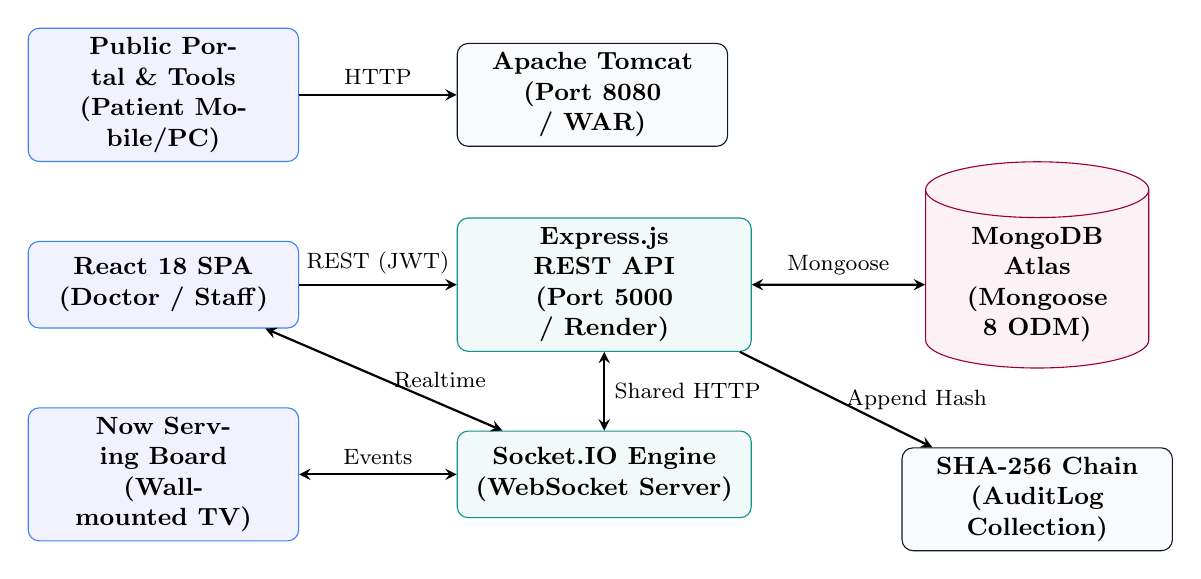
\begin{tikzpicture}[
    node distance=1.5cm and 1.8cm,
    box/.style={rectangle, draw=ctDark, fill=ctBg, rounded corners, text width=3.2cm, minimum height=1.1cm, align=center, font=\small\bfseries},
    clientBox/.style={rectangle, draw=ctAccent, fill=blue!5, rounded corners, text width=3.2cm, minimum height=1.1cm, align=center, font=\small\bfseries},
    serverBox/.style={rectangle, draw=ctPrimary, fill=teal!5, rounded corners, text width=3.5cm, minimum height=1.1cm, align=center, font=\small\bfseries},
    dbBox/.style={cylinder, draw=purple!80!black, fill=purple!5, shape border rotate=90, aspect=0.25, text width=2.6cm, minimum height=1.3cm, align=center, font=\small\bfseries},
    arrow/.style={thick, ->, >=stealth}
]

% Clients
\node[clientBox] (reactClient) {React 18 SPA\\(Doctor / Staff)};
\node[clientBox, below=1.0cm of reactClient] (tvBoard) {Now Serving Board\\(Wall-mounted TV)};
\node[clientBox, above=1.0cm of reactClient] (publicSite) {Public Portal \& Tools\\(Patient Mobile/PC)};

% Web Servers / Gateways
\node[serverBox, right=2.0cm of reactClient] (expressApi) {Express.js REST API\\(Port 5000 / Render)};
\node[serverBox, right=2.0cm of tvBoard] (socketIo) {Socket.IO Engine\\(WebSocket Server)};
\node[box, right=2.0cm of publicSite] (tomcat) {Apache Tomcat\\(Port 8080 / WAR)};

% Database
\node[dbBox, right=2.2cm of expressApi] (mongoDb) {MongoDB Atlas\\(Mongoose 8 ODM)};
\node[box, below=1.0cm of mongoDb] (auditChain) {SHA-256 Chain\\(AuditLog Collection)};

% Connectors
\draw[arrow] (publicSite) -- node[above, font=\footnotesize] {HTTP} (tomcat);
\draw[arrow] (reactClient) -- node[above, font=\footnotesize] {REST (JWT)} (expressApi);
\draw[arrow, <->] (tvBoard) -- node[above, font=\footnotesize] {Events} (socketIo);
\draw[arrow, <->] (reactClient) -- node[right, font=\footnotesize] {Realtime} (socketIo);
\draw[arrow, <->] (expressApi) -- node[right, font=\footnotesize] {Shared HTTP} (socketIo);
\draw[arrow, <->] (expressApi) -- node[above, font=\footnotesize] {Mongoose} (mongoDb);
\draw[arrow] (expressApi) -- node[right, font=\footnotesize] {Append Hash} (auditChain);

\end{tikzpicture}
\caption{ClinicTrack Comprehensive Full-Stack System Architecture}
\label{fig:sys_arch}
\end{figure}

\section{Detailed Operational Workflows}

\subsection{Physician Clinical Consultation Workflow (Git-Style Versioning)}
\begin{enumerate}
    \item \textbf{Authentication:} Physician logs in via \texttt{/login}. The server authenticates credentials against \texttt{bcryptjs} password hashes and issues a signed JSON Web Token (JWT) bearing the \texttt{doctor} role.
    \item \textbf{Patient Lookup \& Selection:} Physician accesses the patient directory (\texttt{/patients}), equipped with dynamic debounce filtering by name or MRN.
    \item \textbf{Consultation Creation ($v_1$):} Doctor records a new visit. The frontend validates fields against \texttt{visitSchema} (ensuring dates are not in the future, vital signs match physiological bounds). The server executes \texttt{express-validator} rules and stores a document in the \texttt{visits} collection:
    $$\{ \text{versionNumber}: 1, \text{familyId}: \text{doc.\_id}, \text{parentVisitId}: \text{null}, \text{isCurrent}: \text{true} \}$$
    \item \textbf{Clinical Amendment ($v_2$ Commit):} If the physician amends notes or alters the diagnosis, the server \textbf{does not update the document in place}. Instead, it sets $v_1$'s \texttt{isCurrent} flag to \texttt{false} and inserts a new document:
    $$\{ \text{versionNumber}: 2, \text{familyId}: v_1.\text{familyId}, \text{parentVisitId}: v_1.\text{\_id}, \text{changeReason}: \text{``Dosage adjusted''} \}$$
    \item \textbf{Visual Diffing \& Rollback:} The physician opens the \texttt{DiffViewer} component. The client displays a side-by-side colorized diff comparing $v_1$ against $v_2$. If $v_2$ was executed erroneously, clicking ``Rollback to this version'' writes an explicit $v_3$ commit marked as a rollback of $v_1$, preserving immutable clinical history.
\end{enumerate}

\subsection{Live Waiting-Room Telemetry Workflow}
\begin{enumerate}
    \item \textbf{Token Issuance:} Desk reception registers arriving patients and clicks ``Issue Token'' on \texttt{/queue}.
    \item \textbf{Atomic Queue Generation:} The backend generates a sequential daily token (e.g., Token \#14 for \texttt{2026-11-02}) stored in the \texttt{queue\_tokens} collection with initial status \texttt{waiting}.
    \item \textbf{WebSocket Event Dispatch:} The controller triggers \texttt{realtimeService.emitQueueUpdated()}, broadcasting a \texttt{queue:token\_created} event to all connected clients.
    \item \textbf{TV Board Refresh:} The wall-mounted display at \texttt{/queue/board} catches the event via its persistent Socket.IO listener and updates the current queue and next-in-line tokens with zero manual DOM reloading.
    \item \textbf{Doctor Call-Out:} The doctor clicks ``Call Next'' in the consultation room. The server transitions the token to \texttt{serving}, recording the \texttt{calledAt} timestamp and immediately flashing Token \#14 onto the TV screen.
\end{enumerate}

\subsection{Prescription Issuance \& Public QR Verification}
\begin{enumerate}
    \item \textbf{Prescription Builder:} Doctor prescribes medicines via \texttt{/patients/:id/prescriptions/new}. The UI enforces medicine dosages (e.g., ``500 mg'') and cross-references patient allergies.
    \item \textbf{Crypto Token Generation:} The server saves the prescription and derives a unique, cryptographically secure 32-character hexadecimal token using \texttt{crypto.randomBytes(16).toString('hex')}.
    \item \textbf{Dynamic PDF Generation:} The doctor clicks ``Download PDF''. Express calls \texttt{pdfkit}, streams binary buffers directly through the HTTP response, and embeds a dynamic QR code pointing to \texttt{https://clinictrack-client.vercel.app/verify/<qrToken>}.
    \item \textbf{Public Verification:} When scanned by a pharmacist or patient, the public route \texttt{/verify/:qrToken} queries the unauthenticated endpoint \texttt{GET /api/prescriptions/verify/:qrToken}, displaying physician details, issue date, and prescribed medicines without exposing internal clinic records.
\end{enumerate}

% =============================================================================
% CHAPTER 4: MAJOR FEATURES & INNOVATIONS
% =============================================================================
\chapter{Major Features \& Technical Innovations}

ClinicTrack integrates several enterprise-grade features that set it apart from standard academic CRUD projects:

\section{Git-Style Electronic Medical Record Versioning}
Medical records cannot ethically or legally be overwritten. ClinicTrack implements a Git-like revision tree directly inside MongoDB:
\begin{itemize}
    \item \textbf{Immutable Visits:} Every modification appends a new document linked to the parent consultation ID.
    \item \textbf{Visual Diff Viewer:} The React frontend computes line-by-line and field-by-field differences, rendering additions in green badge containers and deletions in struck-through red containers.
    \item \textbf{Non-Destructive Rollback:} A rollback creates a forward copy of the target historical version, maintaining an unbroken chronological chain of edits.
\end{itemize}

\section{Cryptographic SHA-256 Tamper-Evident Audit Chain}
To satisfy healthcare compliance standards, ClinicTrack implements a cryptographic hash chain inspired by blockchain data structures. 

\subsection{Mathematical Hash Formulations}
Each audit entry $E_i$ stores an audited-at timestamp $T_i$, actor ID $A_i$, action string $C_i$, target entity $X_i$, and previous hash $H_{i-1}$. The entry's hash $H_i$ is computed as:
\begin{equation}
    H_0 = \text{``GENESIS''}
\end{equation}
\begin{equation}
    H_i = \text{SHA-256}\Big(H_{i-1} + \text{CanonicalJSON}\big(\{C_i, X_i, A_i, T_i\}\big)\Big)
\end{equation}

Figure~\ref{fig:hash_chain} illustrates the sequential cryptographic dependency of the audit trail.

\begin{figure}[h!]
\centering
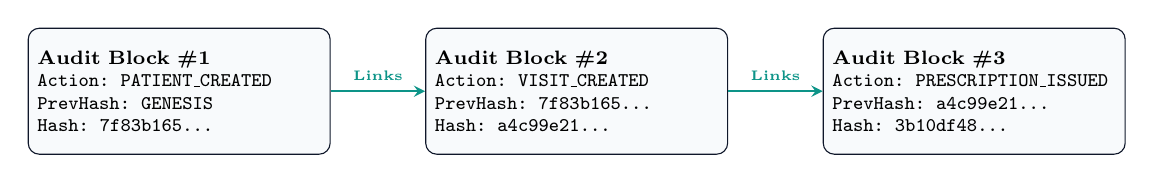
\begin{tikzpicture}[
    node distance=1.0cm,
    block/.style={rectangle, draw=ctDark, fill=ctBg, rounded corners, text width=3.6cm, minimum height=1.6cm, align=left, font=\scriptsize},
    arrow/.style={thick, ->, >=stealth, color=ctPrimary}
]

\node[block] (block1) {
    \textbf{Audit Block \#1} \\
    \texttt{Action: PATIENT\_CREATED} \\
    \texttt{PrevHash: GENESIS} \\
    \texttt{Hash: 7f83b165...}
};

\node[block, right=1.2cm of block1] (block2) {
    \textbf{Audit Block \#2} \\
    \texttt{Action: VISIT\_CREATED} \\
    \texttt{PrevHash: 7f83b165...} \\
    \texttt{Hash: a4c99e21...}
};

\node[block, right=1.2cm of block2] (block3) {
    \textbf{Audit Block \#3} \\
    \texttt{Action: PRESCRIPTION\_ISSUED} \\
    \texttt{PrevHash: a4c99e21...} \\
    \texttt{Hash: 3b10df48...}
};

\draw[arrow] (block1) -- node[above, font=\tiny\bfseries] {Links} (block2);
\draw[arrow] (block2) -- node[above, font=\tiny\bfseries] {Links} (block3);

\end{tikzpicture}
\caption{Cryptographic SHA-256 Audit Chain Architecture}
\label{fig:hash_chain}
\end{figure}

\subsection{Live In-Browser Verification Engine}
On the \texttt{/audit} screen, the system provides a \textbf{``Verify Integrity''} button. Clicking it initiates a client-side execution loop that retrieves the audit log and independently re-hashes every link using the browser's native Web Crypto API:
$$\text{RecomputedHash}_i \stackrel{?}{=} \text{StoredHash}_i \quad \wedge \quad \text{StoredPrevHash}_i \stackrel{?}{=} \text{StoredHash}_{i-1}$$
If any record in MongoDB has been altered directly via database GUI or CLI tools, the chain breaks at that exact index, instantly highlighting the compromised row in red with a forensic discrepancy report.

\section{Live Waiting-Room Queue \& Now Serving TV Board}
\begin{itemize}
    \item \textbf{Token State Machine:} Tokens advance deterministically: $\text{waiting} \rightarrow \text{serving} \rightarrow \text{done}$ (or $\text{skipped}$).
    \item \textbf{Dual-Screen Layout:} Reception and consulting doctors use the operational queue console (\texttt{/queue}), while the waiting lobby runs the full-screen ``Now Serving'' board (\texttt{/queue/board}) designed with large-format typography for viewing from 20+ feet away.
    \item \textbf{Real-Time Synchronization:} Socket.IO WebSocket broadcasts notify all listening clients in $<15\text{ ms}$, eliminating server polling overhead.
\end{itemize}

\section{Prescription Builder with Streaming PDF \& Public QR Verification}
\begin{itemize}
    \item \textbf{In-Memory Binary Streaming:} Prescription PDFs are generated on the fly via Node.js streams and \texttt{pdfkit}, piping directly into HTTP response streams without writing temporary files to the server's disk.
    \item \textbf{Tamper-Proof QR Code:} Every printed prescription features an embedded high-resolution QR code encoding a secure public URL. Scanning it allows any pharmacy or patient to verify authenticity without requiring clinic staff login credentials.
\end{itemize}

\section{Clinical Intelligence Analytics Dashboard}
The \texttt{/analytics} module delivers real-time clinical telemetry powered by server-side MongoDB aggregation pipelines (no counting in JavaScript):
\begin{itemize}
    \item 14-day patient consultation volume trend graphs (SVG area chart).
    \item Top 5 clinical diagnoses distribution (bar charts).
    \item Peak clinic arrival hours breakdown (hourly density histograms).
    \item Ratio of new vs. returning patient retention.
\end{itemize}

\section{Role-Based Access Control (RBAC) \& Safety Alerts}
\begin{itemize}
    \item \textbf{Strict Role Segregation:} The system distinguishes three roles: \texttt{doctor}, \texttt{staff} (reception), and \texttt{admin}. Reception staff can register demographics and issue queue tokens, but the backend strictly returns \texttt{403 Forbidden} if they attempt to access clinical notes, diagnoses, or prescriptions.
    \item \textbf{Allergy Cross-Alert:} When a physician selects a patient with documented drug sensitivities, the consultation and prescription screens highlight prominent high-contrast alerts to prevent adverse prescribing events.
\end{itemize}

% =============================================================================
% CHAPTER 5: DATABASE DESIGN & SCHEMA ARCHITECTURE
% =============================================================================
\chapter{Database Design \& Schemas}
\label{chap:database}

\section{Database Technology Selection: MongoDB \& Mongoose ODM}
ClinicTrack uses **MongoDB** as its primary persistence engine, interfaced via the **Mongoose 8** Object Data Modeling (ODM) library. The document-oriented NoSQL model was chosen over relational databases because:
\begin{enumerate}
    \item \textbf{Flexible Consultation Documents:} Medical visits vary widely in structure (e.g., pediatric visits require weight-based dosages, while cardiology visits record multi-field blood pressure, heart rate, and ECG notes). Storing these in dynamic JSON/BSON structures avoids sparse, unmaintainable SQL tables with dozens of nullable columns.
    \item \textbf{Embedded Arrays for Versioning:} A visit's complete revision history, symptoms list, and prescribed medicine items are naturally modeled as structured embedded arrays and sub-documents.
    \item \textbf{Aggregation Pipeline Power:} MongoDB's aggregation framework processes complex statistical groupings (e.g., peak arrival hours and daily visit trends) natively in the database engine with minimal memory consumption.
\end{enumerate}

\section{Data Dictionary \& Schema Specifications}

\subsection{\texttt{User} Schema (Authentication \& Roles)}
Represents authenticated clinical personnel. Passwords are encrypted using \texttt{bcryptjs} with a work factor of 10 and excluded from query results by default (\texttt{select: false}).
\begin{table}[h!]
\centering
\caption{User Collection Schema Specification}
\small
\begin{tabularx}{\textwidth}{l l l X}
\toprule
\textbf{Field Name} & \textbf{BSON Type} & \textbf{Constraints} & \textbf{Description} \\
\midrule
\texttt{\_id} & ObjectId & Primary Key & Unique user identifier \\
\texttt{name} & String & Required, Trim & Full legal name of the staff member / doctor \\
\texttt{email} & String & Required, Unique, Lower & Email address utilized as login username \\
\texttt{password} & String & Required, \texttt{select: false} & Salted bcrypt password hash \\
\texttt{role} & String & Enum [\texttt{doctor}, \texttt{staff}, \texttt{admin}] & Role for Role-Based Access Control (RBAC) \\
\texttt{specialty} & String & Optional, Trim & Medical specialty (e.g., General Medicine) \\
\texttt{createdAt} & Date & Auto-timestamp & Account creation timestamp \\
\bottomrule
\end{tabularx}
\end{table}

\subsection{\texttt{Patient} Schema (Demographics \& Records)}
Represents a patient registered at the clinic. Enforces unique auto-incrementing Medical Record Numbers (MRN) via a Mongoose \texttt{pre('save')} hook.
\begin{table}[h!]
\centering
\caption{Patient Collection Schema Specification}
\small
\begin{tabularx}{\textwidth}{l l l X}
\toprule
\textbf{Field Name} & \textbf{BSON Type} & \textbf{Constraints} & \textbf{Description} \\
\midrule
\texttt{\_id} & ObjectId & Primary Key & Internal unique patient identifier \\
\texttt{mrn} & String & Unique, Indexed & Formatted Medical Record Number (e.g., \texttt{MC-00017}) \\
\texttt{fullName} & String & Required, Regex & Patient legal full name \\
\texttt{phone} & String & Required, Regex & 10-digit Indian mobile number ($[6-9]\backslash d^9$) \\
\texttt{dob} & Date & Required, Past Date & Date of birth (computes virtual \texttt{age}) \\
\texttt{gender} & String & Enum [\texttt{male}, \texttt{female}, \texttt{other}] & Biological gender \\
\texttt{bloodGroup} & String & Enum [\texttt{A+}, \texttt{O+}, \dots, \texttt{AB-}] & Patient blood type \\
\texttt{allergies} & Array[String] & Clinical Access Only & Known drug / food allergies \\
\texttt{treatment} & String & Max 300 chars & Primary reason for consultation \\
\texttt{primaryDoctorId}& ObjectId & Ref: \texttt{User} & Assigned consulting physician \\
\bottomrule
\end{tabularx}
\end{table}

\subsection{\texttt{Visit} Schema (Version-Tracked Clinical Record)}
Models an individual consultation version. Edits append a new document sharing the same \texttt{familyId} with an incremented \texttt{versionNumber}.
\begin{table}[h!]
\centering
\caption{Visit Collection Schema Specification}
\small
\begin{tabularx}{\textwidth}{l l l X}
\toprule
\textbf{Field Name} & \textbf{BSON Type} & \textbf{Constraints} & \textbf{Description} \\
\midrule
\texttt{\_id} & ObjectId & Primary Key & Unique visit version identifier \\
\texttt{patientId} & ObjectId & Ref: \texttt{Patient}, Indexed & Foreign key to parent patient \\
\texttt{doctorId} & ObjectId & Ref: \texttt{User}, Required & Physician who conducted consultation \\
\texttt{visitDate} & Date & Required, Non-future & Date and time of consultation \\
\texttt{diagnosis} & String & Required, 2--200 chars & Medical diagnostic finding \\
\texttt{symptoms} & Array[String] & Trimmed & List of presenting symptoms \\
\texttt{notes} & String & Max 4000 chars & Confidential clinical observation notes \\
\texttt{vitals} & Subdocument & Temp, BP, Pulse & Measured vital signs \\
\texttt{familyId} & ObjectId & Indexed & Root version ID uniting all revisions \\
\texttt{versionNumber} & Number & Required, Min: 1 & Revision number ($1, 2, 3, \dots$) \\
\texttt{parentVisitId} & ObjectId & Ref: \texttt{Visit} & ID of the preceding version \\
\texttt{isCurrent} & Boolean & Default: \texttt{true}, Indexed & Flag denoting the active, latest version \\
\texttt{changeReason} & String & Required for $v > 1$ & Clinical rationale for the amendment \\
\bottomrule
\end{tabularx}
\end{table}

\subsection{\texttt{QueueToken} Schema (Live Telemetry)}
Maintains daily waiting room queues with guaranteed uniqueness per day.
\begin{table}[h!]
\centering
\caption{QueueToken Collection Schema Specification}
\small
\begin{tabularx}{\textwidth}{l l l X}
\toprule
\textbf{Field Name} & \textbf{BSON Type} & \textbf{Constraints} & \textbf{Description} \\
\midrule
\texttt{\_id} & ObjectId & Primary Key & Unique token document ID \\
\texttt{dayKey} & String & Format: \texttt{YYYY-MM-DD} & Current date identifier (restarts daily) \\
\texttt{tokenNumber} & Number & Required, Min: 1 & Sequential token ticket number \\
\texttt{patientId} & ObjectId & Ref: \texttt{Patient} & Patient awaiting consultation \\
\texttt{doctorId} & ObjectId & Ref: \texttt{User} & Consulting doctor assigned to patient \\
\texttt{status} & String & Enum: \texttt{waiting, serving,} & Current token lifecycle state \\
& & \texttt{done, skipped} & \\
\texttt{calledAt} & Date & Optional & Timestamp when token was announced \\
\texttt{completedAt} & Date & Optional & Timestamp when consultation finished \\
\bottomrule
\end{tabularx}
\end{table}

\subsection{\texttt{AuditLog} Schema (Cryptographic SHA-256 Chain)}
Maintains an immutable, append-only security trail.
\begin{table}[h!]
\centering
\caption{AuditLog Collection Schema Specification}
\small
\begin{tabularx}{\textwidth}{l l l X}
\toprule
\textbf{Field Name} & \textbf{BSON Type} & \textbf{Constraints} & \textbf{Description} \\
\midrule
\texttt{\_id} & ObjectId & Primary Key & Unique audit entry ID \\
\texttt{actorId} & ObjectId & Ref: \texttt{User} & User executing the action \\
\texttt{action} & String & Required, Indexed & Action performed (e.g., \texttt{VISIT\_CREATED}) \\
\texttt{entity} & String & Required & Entity modified (\texttt{Patient}, \texttt{Visit}) \\
\texttt{entityId} & String & Required & Target entity ID \\
\texttt{at} & Date & Required & Canonical audited timestamp \\
\texttt{prevHash} & String & Required & Hash of immediately preceding log record \\
\texttt{hash} & String & Unique, Required & SHA-256 hash computed over this entry \\
\bottomrule
\end{tabularx}
\end{table}

\section{Database Indexing \& Performance Optimization}
To support rapid read queries on high-volume clinic days, compound indexes are defined:
\begin{itemize}
    \item \texttt{visitSchema.index(\{ patientId: 1, isCurrent: 1 \})}: Accelerates dashboard queries retrieving the current active consultation of a patient in $O(\log N)$ index scan time without scanning historic drafts.
    \item \texttt{queueTokenSchema.index(\{ dayKey: 1, tokenNumber: 1 \}, \{ unique: true \})}: Prevents duplicate token collisions during simultaneous receptionist ticket generation.
    \item \texttt{patientSchema.index(\{ phone: 1 \})}: Enables near-instant lookups when checking in returning patients by mobile number.
\end{itemize}

\section{Comparative Database Study: MongoDB vs. DynamoDB vs. Cassandra}
In fulfillment of the syllabus self-study criteria, Table~\ref{tab:db_comparison} details how MongoDB compares with Amazon DynamoDB and Apache Cassandra.

\begin{table}[h!]
\centering
\caption{Comparative Architectural Analysis of NoSQL Databases}
\label{tab:db_comparison}
\small
\begin{tabularx}{\textwidth}{p{3.0cm} X X X}
\toprule
\textbf{Dimension} & \textbf{MongoDB (ClinicTrack)} & \textbf{Amazon DynamoDB} & \textbf{Apache Cassandra} \\
\midrule
\textbf{Data Model} & Document-oriented (JSON / BSON documents) & Key-Value and Document store & Wide-Column distributed family store \\
\midrule
\textbf{Schema Flexibility} & Dynamic / Schema-optional with Mongoose enforcement & Dynamic attributes per Partition Key & Rigid tabular column families defined via CQL \\
\midrule
\textbf{Query Capabilities} & Rich queries, regex, multi-stage aggregation pipeline & Primary/Sort key lookups; filtered secondary index scans & Fast lookups on partition keys; no ad-hoc joins/aggregations \\
\midrule
\textbf{Architecture} & Primary-Replica replica set with configurable sharding & Fully managed serverless proprietary AWS service & Decentralized masterless (Peer-to-Peer) ring topology \\
\midrule
\textbf{CAP Theorem} & CP (Consistency \& Partition Tolerance) & Configurable (Eventual or Strong consistency per read) & AP (High Availability \& Partition Tolerance, Tunable) \\
\midrule
\textbf{Primary Use Case} & Complex clinical records, nested arrays, analytics & High-scale cloud-native key-value workloads & Massive write-heavy time-series and IoT telemetry \\
\bottomrule
\end{tabularx}
\end{table}

% =============================================================================
% CHAPTER 6: TWO-TIER VALIDATION ARCHITECTURE
% =============================================================================
\chapter{Two-Tier Validation Strategy}

ClinicTrack enforces a rigorous **Two-Tier Validation Architecture**. Client-side validation improves User Experience (UX) through instant feedback, while Server-side validation guarantees Security and Data Integrity against bypassed browser environments.

\begin{figure}[h!]
\centering
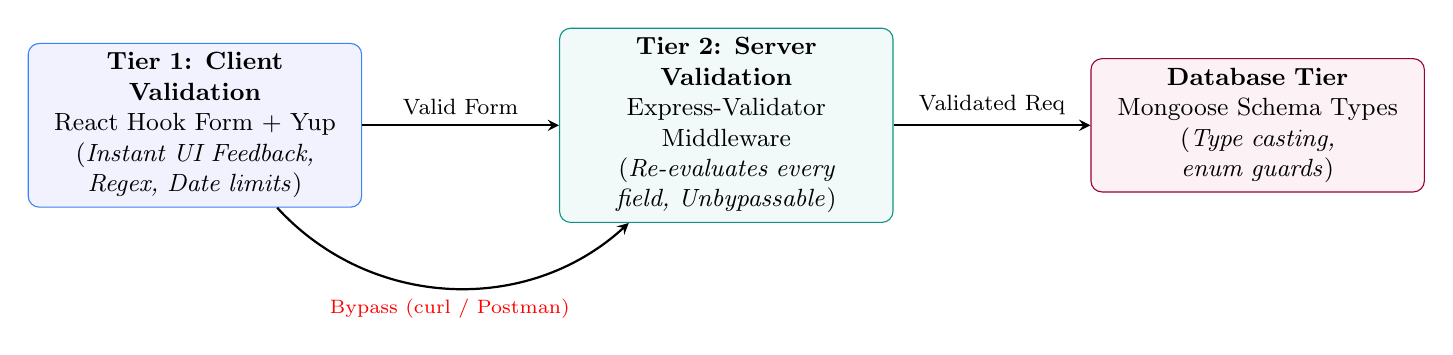
\begin{tikzpicture}[
    node distance=1.5cm and 2.5cm,
    block/.style={rectangle, draw=ctDark, fill=ctBg, rounded corners, text width=4.0cm, minimum height=1.3cm, align=center, font=\small},
    arrow/.style={thick, ->, >=stealth}
]

\node[block, draw=ctAccent, fill=blue!5] (client) {\textbf{Tier 1: Client Validation}\\React Hook Form + Yup\\(\textit{Instant UI Feedback, Regex, Date limits})};
\node[block, draw=ctPrimary, fill=teal!5, right=of client] (server) {\textbf{Tier 2: Server Validation}\\Express-Validator Middleware\\(\textit{Re-evaluates every field, Unbypassable})};
\node[block, draw=purple!80!black, fill=purple!5, right=of server] (db) {\textbf{Database Tier}\\Mongoose Schema Types\\(\textit{Type casting, enum guards})};

\draw[arrow] (client) -- node[above, font=\footnotesize] {Valid Form} (server);
\draw[arrow] (server) -- node[above, font=\footnotesize] {Validated Req} (db);
\draw[arrow] (client) edge[bend right=45] node[below, font=\scriptsize\color{red}] {Bypass (curl / Postman)} (server);

\end{tikzpicture}
\caption{Two-Tier Defense-in-Depth Validation Pipeline}
\label{fig:validation_pipeline}
\end{figure}

\section{Comparison of Client-Side vs. Server-Side Validation}
\begin{table}[h!]
\centering
\caption{Comparative Matrix: Tier 1 vs. Tier 2 Validation}
\label{tab:validation_comparison}
\begin{tabularx}{\textwidth}{p{3.5cm} X X}
\toprule
\textbf{Evaluation Factor} & \textbf{Tier 1: Client-Side (Yup)} & \textbf{Tier 2: Server-Side (express-validator)} \\
\midrule
\textbf{Primary Purpose} & User Experience (UX), immediate input feedback & Data Security, regulatory compliance, integrity \\
\textbf{Execution Point} & Browser JavaScript runtime before network request & Express middleware pipeline before controller execution \\
\textbf{Bypass Vulnerability} & Easily bypassed (disabling JS, curl, Postman) & Cannot be bypassed by external API callers \\
\textbf{Error Presentation} & Inline red error badges under individual fields & Standard HTTP 422 Unprocessable Entity JSON \\
\textbf{Performance Impact} & Prevents unnecessary network requests to server & Protects database against malformed queries \\
\bottomrule
\end{tabularx}
\end{table}

\section{Implementation Code Comparison}

\subsection{Client-Side Validation Implementation (React Hook Form + Yup)}
The following snippet from \texttt{client/src/validation/schemas.js} highlights the declarative patient validation rules:

\begin{lstlisting}[language=JavaScript, caption={Client-Side Yup Patient Validation Schema}]
export const patientSchema = yup.object({
  fullName: yup.string().trim()
    .required('Full name is required')
    .matches(/^[A-Za-z][A-Za-z .-]{1,58}$/, 'Letters, spaces, dots and hyphens only'),
  phone: yup.string().trim()
    .required('Mobile number is required')
    .matches(/^[6-9]\d{9}$/, 'Enter a 10-digit Indian mobile number starting with 6-9'),
  dob: yup.string()
    .required('Date of birth is required')
    .test('not-future', 'Date of birth cannot be in the future', 
          v => !v || v <= todayISO()),
  gender: yup.string()
    .oneOf(['male', 'female', 'other'], 'Select a valid gender')
    .required('Select a gender'),
  treatment: yup.string()
    .max(300, 'Keep treatment details under 300 characters').optional(),
  allergies: yup.string()
    .max(200, 'Keep allergies under 200 characters').optional()
});
\end{lstlisting}

\subsection{Server-Side Validation Implementation (express-validator)}
The following snippet from \texttt{server/routes/patient.routes.js} demonstrates independent server-side re-verification:

\begin{lstlisting}[language=JavaScript, caption={Server-Side express-validator Rules}]
const patientRules = [
  body('fullName')
    .matches(/^[A-Za-z][A-Za-z .-]{1,58}$/)
    .withMessage('Name must be letters, spaces, dots or hyphens'),
  body('phone')
    .matches(/^[6-9]\d{9}$/)
    .withMessage('Indian mobile: 10 digits starting with 6-9'),
  body('dob')
    .isISO8601().withMessage('Date of birth must be a valid date (YYYY-MM-DD)')
    .custom(v => new Date(v) < new Date()).withMessage('DOB cannot be in the future'),
  body('gender')
    .isIn(['male', 'female', 'other']).withMessage('gender must be male/female/other'),
  body('allergies')
    .optional().isArray().withMessage('allergies must be an array of strings')
];

// Route attachment via validation wrapper
router.post('/', authorize('doctor', 'staff', 'admin'), validate(patientRules), createPatient);
\end{lstlisting}

\subsection{Centralized Validation Middleware Wrapper}
In \texttt{server/middleware/validate.js}, a reusable higher-order middleware collects all validation errors and formats a uniform error response:
\begin{lstlisting}[language=JavaScript, caption={Centralized Validation Middleware Wrapper}]
function validate(rules) {
  const handleResult = (req, res, next) => {
    const result = validationResult(req);
    if (!result.isEmpty()) {
      return next(
        new HttpError(
          422,
          'Validation failed',
          result.array().map(e => ({ field: e.path, message: e.msg }))
        )
      );
    }
    return next();
  };
  return [...rules, handleResult];
}
\end{lstlisting}

% =============================================================================
% CHAPTER 7: RESTFUL APIS, SECURITY & CLOUD DEPLOYMENT
% =============================================================================
\chapter{RESTful APIs, Security \& Cloud Deployment}

\section{RESTful API Design \& Catalog}
The backend delivers 30+ endpoints designed according to REST principles. Every endpoint returns predictable JSON envelopes:
\begin{itemize}
    \item \textbf{Success Envelope:} \texttt{\{ success: true, data: ..., meta: \{ page, limit, total \} \}}
    \item \textbf{Error Envelope:} \texttt{\{ success: false, message: "...", errors: [...] \}}
\end{itemize}

Table~\ref{tab:api_catalogue} enumerates the primary REST endpoints organized by clinical resource.

\begin{table}[h!]
\centering
\caption{Core RESTful API Endpoint Catalogue}
\label{tab:api_catalogue}
\small
\begin{tabularx}{\textwidth}{l l p{3.2cm} X}
\toprule
\textbf{HTTP Method} & \textbf{Endpoint Path} & \textbf{Authorized Roles} & \textbf{Operation / Description} \\
\midrule
\texttt{POST} & \texttt{/api/auth/login} & Public (Rate-limited) & Authenticate user, issue signed JWT \\
\texttt{GET}  & \texttt{/api/auth/me} & All authenticated & Retrieve currently logged-in user profile \\
\midrule
\texttt{GET}  & \texttt{/api/patients} & Doctor, Staff, Admin & Paginated patient list with search filter \\
\texttt{POST} & \texttt{/api/patients} & Doctor, Staff, Admin & Register new patient demographics \\
\texttt{GET}  & \texttt{/api/patients/:id} & Doctor, Staff, Admin & Retrieve individual patient record \\
\texttt{PUT}  & \texttt{/api/patients/:id} & Doctor, Admin & Update demographic details \\
\midrule
\texttt{POST} & \texttt{/api/patients/:id/visits} & Doctor, Admin & Create initial visit or append new version \\
\texttt{GET}  & \texttt{/api/patients/:id/visits} & Doctor, Admin & Retrieve complete versioned visit history \\
\texttt{POST} & \texttt{/api/.../visits/:vId/rollback} & Doctor, Admin & Restore an earlier consultation revision \\
\midrule
\texttt{POST} & \texttt{/api/prescriptions} & Doctor, Admin & Issue medicine prescription \\
\texttt{GET}  & \texttt{/api/prescriptions/:id/pdf} & Doctor, Admin & Stream downloadable prescription PDF \\
\texttt{GET}  & \texttt{/api/prescriptions/verify/:qr} & Public (No auth) & Public digital QR verification \\
\midrule
\texttt{GET}  & \texttt{/api/queue} & Doctor, Staff, Admin & Retrieve active daily waiting queue \\
\texttt{POST} & \texttt{/api/queue} & Doctor, Staff, Admin & Issue new waiting-room ticket token \\
\texttt{PATCH}& \texttt{/api/queue/:id/status} & Doctor, Staff, Admin & Transition state (waiting $\rightarrow$ serving $\rightarrow$ done) \\
\midrule
\texttt{GET}  & \texttt{/api/audit} & Doctor, Admin & Retrieve SHA-256 chained audit logs \\
\texttt{GET}  & \texttt{/api/analytics/summary} & Doctor, Admin & Retrieve MongoDB aggregation metrics \\
\bottomrule
\end{tabularx}
\end{table}

\section{Security Architecture \& Defense-in-Depth}
\begin{enumerate}
    \item \textbf{Stateless JWT Authentication:} JSON Web Tokens signed with HMAC-SHA256 (\texttt{HS256}) authenticate requests via HTTP header \texttt{Authorization: Bearer <token>}. The server verifies token signatures cryptographically without requiring server-side session lookups.
    \item \textbf{HTTP Security Headers (\texttt{helmet}):} Enforces secure headers, including HTTP Strict Transport Security (HSTS), X-Content-Type-Options (\texttt{nosniff}), and X-Frame-Options (\texttt{DENY}) to thwart clickjacking and MIME-type sniffing.
    \item \textbf{Brute-Force Rate Limiting (\texttt{express-rate-limit}):} Login attempts are restricted to a maximum of 20 requests per 15 minutes per IP address, while general API traffic is throttled to 500 requests per 15 minutes.
    \item \textbf{Cross-Origin Resource Sharing (CORS):} The Express server explicitly whitelists the React client domain (\texttt{CLIENT\_URL}) and blocks untrusted cross-origin requests.
\end{enumerate}

\section{Cloud Deployment Architecture}
The application is deployed across specialized cloud providers to achieve high availability, low latency, and continuous delivery:

\begin{table}[h!]
\centering
\caption{Production Cloud Deployment Infrastructure}
\label{tab:deployment_matrix}
\begin{tabularx}{\textwidth}{l l l X}
\toprule
\textbf{Sub-System} & \textbf{Cloud Platform} & \textbf{Runtime Environment} & \textbf{Deployment Link / Endpoint} \\
\midrule
\textbf{React Client} & Vercel & Static Vite SPA on Edge CDN & \url{https://clinictrack-client.vercel.app} \\
\textbf{Express API}  & Render & Node.js Web Service (LTS) & \url{https://clinictrack-api.onrender.com} \\
\textbf{Database}     & MongoDB Atlas & Cloud M0 Cluster (Mumbai) & \texttt{mongodb+srv://...@cluster0.mongodb.net} \\
\textbf{Public Site}  & Apache Tomcat & Java EE Exploded WAR / Webapp & \url{http://localhost:8080/clinictrack/} \\
\bottomrule
\end{tabularx}
\end{table}

\subsection{Apache Tomcat Deployment of Public Marketing Site}
In accordance with Practical No.~01, the static public site and diagnostic tools are packaged for Apache Tomcat web server:
\begin{enumerate}
    \item Configured \texttt{public-site/WEB-INF/web.xml} with standard deployment descriptors:
\begin{lstlisting}[language=XML, caption={Apache Tomcat web.xml Deployment Descriptor}]
<?xml version="1.0" encoding="UTF-8"?>
<web-app xmlns="http://xmlns.jcp.org/xml/ns/javaee" version="3.1">
  <display-name>ClinicTrack Public Website</display-name>
  <welcome-file-list>
    <welcome-file>index.html</welcome-file>
  </welcome-file-list>
</web-app>
\end{lstlisting}
    \item Deployed the directory into Tomcat's \texttt{webapps/clinictrack/} directory or bundled as \texttt{clinictrack.war} via \texttt{jar -cvf clinictrack.war *}.
    \item Started Tomcat via \texttt{bin/startup.sh}. The site is accessible at \texttt{http://localhost:8080/clinictrack/}.
\end{enumerate}

% =============================================================================
% CHAPTER 8: INDIVIDUAL DEMONSTRATION & PRESENTATION GUIDE
% =============================================================================
\chapter{Individual Demonstration \& Presentation Guide}

To satisfy the academic evaluation criteria where each student presents and demonstrates their contributions individually, this chapter defines the precise demonstration sequence, walkthrough scripts, and code navigation coordinates for each team member.

\section{Student 1: Nupoor Deshpande (PRN: 202401100026)}
\paragraph{Assigned Core Topics:} Backend Architecture, Express Middleware Pipeline, MongoDB Schemas \& Aggregation, Server Validation, and REST APIs.

\subsection{Demonstration Checklist}
\begin{enumerate}
    \item \textbf{Express Server Initialization:} Open \texttt{server/app.js}. Explain the middleware sequence: \texttt{helmet()} $\rightarrow$ \texttt{cors()} $\rightarrow$ \texttt{rateLimit()} $\rightarrow$ \texttt{express.json()} $\rightarrow$ route registration $\rightarrow$ centralized \texttt{HttpError} handler.
    \item \textbf{Server-Side Validation:} Open \texttt{server/middleware/validate.js} and \texttt{server/routes/patient.routes.js}. Show how \texttt{patientRules} validates regex patterns for Indian phone numbers ($[6-9]\backslash d^9$) and ensures dates of birth cannot be in the future.
    \item \textbf{MongoDB Aggregation Demonstration:} Open \texttt{server/controllers/analytics.controller.js}. Walk through the multi-stage aggregation pipeline calculating monthly patient arrivals using \texttt{\$match}, \texttt{\$group}, \texttt{\$dateToString}, and \texttt{\$count}.
    \item \textbf{Postman API Testing:} Import \texttt{docs/clinictrack.postman\_collection.json} into Postman. Execute \texttt{POST /api/auth/login}, show how the test script automatically extracts the JWT token into \texttt{\{\{token\}\}}, and execute an authenticated \texttt{GET /api/patients} request.
\end{enumerate}

\section{Student 2: Bhoomi Tiple (PRN: 202401100027)}
\paragraph{Assigned Core Topics:} React 18 SPA Architecture, Client Validation (Yup + RHF), Git-Style EMR Timeline, and Diff Viewer UI.

\subsection{Demonstration Checklist}
\begin{enumerate}
    \item \textbf{React SPA Shell \& Routing:} Open \texttt{client/src/App.jsx}. Explain the client-side routing structure, nested dashboard layouts, and demonstrate how \texttt{<ProtectedRoute allowedRoles=\{['doctor']\}>} prevents unauthorized reception staff from accessing clinical pages.
    \item \textbf{Client-Side Validation in Action:} Open \texttt{client/src/pages/PatientRegister.jsx} and \texttt{client/src/validation/schemas.js}. Type an invalid phone number or future birth date in the UI; show the instant red error badge generated without submitting to the server.
    \item \textbf{Git-Style Visit Versioning \& Diff Viewer:} Navigate to a patient profile in the browser. Add an amended diagnosis to an existing visit. Open the \texttt{DiffViewer} screen and demonstrate the side-by-side view highlighting modified fields in green and red.
    \item \textbf{Analytics Dashboard Visuals:} Open \texttt{client/src/pages/Analytics.jsx}. Demonstrate the responsive SVG charts rendered via \texttt{Recharts} displaying live data fetched from the backend aggregation endpoint.
\end{enumerate}

\section{Student 3: Janhavi Hinganghatkar (PRN: 202401100025)}
\paragraph{Assigned Core Topics:} Real-Time Socket.IO Telemetry, Cryptographic SHA-256 Audit Chain, PDF Streaming, Public Verification, and Tomcat Deployment.

\subsection{Demonstration Checklist}
\begin{enumerate}
    \item \textbf{Live Waiting Queue \& TV Board Demo:} Open two browser windows side by side: the reception console at \texttt{/queue} and the TV board at \texttt{/queue/board}. Issue a new token in window 1; show window 2 updating instantaneously over Socket.IO WebSockets without refreshing.
    \item \textbf{Cryptographic Audit Chain \& Live Verification:} Open \texttt{server/services/audit.service.js}. Explain the SHA-256 formulation. Open \texttt{/audit} in the browser and click the \textbf{``Verify Integrity''} button; demonstrate the in-browser hash re-calculation showing 100\% mathematical integrity.
    \item \textbf{PDF Prescription Generation \& QR Code:} Issue a prescription for a patient. Click ``Download PDF''; inspect the generated PDFKit document with doctor credentials and the scannable QR code. Open the public verification URL \texttt{/verify/:qrToken} to show zero-login authentication.
    \item \textbf{Public Marketing Site on Tomcat:} Open \texttt{public-site/index.html} deployed on Apache Tomcat (\texttt{http://localhost:8080/clinictrack/}). Demonstrate the interactive BMI and Pediatric Dose calculators built with vanilla JavaScript.
\end{enumerate}

% =============================================================================
% CHAPTER 9: COMPREHENSIVE VIVA VOCE QUESTIONS & MODEL ANSWERS
% =============================================================================
\chapter{Comprehensive Viva Voce Preparation}

This chapter compiles the top technical viva questions mapped directly to the 7 syllabus practicals, providing concise, examiner-targeted model answers.

\section{Topic 1: HTML5, CSS3, Bootstrap 5 \& Apache Tomcat}
\paragraph{Q1: What are HTML5 Semantic Elements and why are they used in ClinicTrack?}
\textbf{Answer:} Semantic elements (such as \texttt{<header>}, \texttt{<nav>}, \texttt{<main>}, \texttt{<section>}, \texttt{<article>}, \texttt{<footer>}) clearly state their meaning to browsers, developers, and search engines. They improve SEO rankings, provide landmarks for screen reader accessibility (a11y), and eliminate unmaintainable ``div soup''.

\paragraph{Q2: How does Bootstrap 5 achieve responsiveness?}
\textbf{Answer:} Bootstrap 5 uses a mobile-first 12-column flexbox grid. Viewports are partitioned using CSS media queries into standard breakpoints: \texttt{xs} ($<576\text{px}$), \texttt{sm} ($\ge 576\text{px}$), \texttt{md} ($\ge 768\text{px}$), \texttt{lg} ($\ge 992\text{px}$), \texttt{xl} ($\ge 1200\text{px}$). Column classes (e.g., \texttt{col-12 col-md-6 col-lg-4}) adapt dynamically to screen widths.

\paragraph{Q3: What is Apache Tomcat and how is the public site deployed to it?}
\textbf{Answer:} Apache Tomcat is an open-source Java Servlet Container and HTTP web server. We configured a Java EE deployment descriptor (\texttt{WEB-INF/web.xml}) specifying \texttt{index.html} in the \texttt{<welcome-file-list>}, copied the assets to \texttt{webapps/clinictrack/}, and launched Tomcat on port 8080.

\section{Topic 2: Vanilla JavaScript, DOM Manipulation \& JSON Stores}
\paragraph{Q4: What is the DOM and how does JavaScript manipulate it?}
\textbf{Answer:} The Document Object Model (DOM) is an in-memory, tree-structured object representation of an HTML document created by the browser. JavaScript uses methods like \texttt{document.getElementById}, \texttt{querySelector}, and \texttt{addEventListener} to dynamically update content, styles, and nodes without page reloads.

\paragraph{Q5: What is Event Delegation and why is it useful?}
\textbf{Answer:} Event delegation is a technique where a single event listener is attached to a parent element rather than attaching separate listeners to multiple child elements. It leverages \textbf{Event Bubbling} (events propagating up the DOM tree), drastically reducing memory consumption and supporting dynamically added child elements.

\section{Topic 3: Front-End Framework: ReactJS}
\paragraph{Q6: What is the Virtual DOM and how does React reconciliation work?}
\textbf{Answer:} The Virtual DOM is a lightweight in-memory representation of the real DOM. When component state changes, React renders a new Virtual DOM tree, executes a diffing algorithm comparing it against the previous snapshot, calculates the minimal set of changes, and batches updates to the real DOM to prevent costly layout reflows.

\paragraph{Q7: Why use React Hook Form + Yup over standard React \texttt{useState}?}
\textbf{Answer:} Standard controlled components trigger a component re-render on \textit{every keystroke}, degrading performance in large forms. \texttt{react-hook-form} uses uncontrolled inputs via native DOM refs, isolating re-renders strictly to validation status updates. Yup decouples declarative validation schemas into clean, reusable objects.

\section{Topic 4: Server-Side Development: Node.js}
\paragraph{Q8: Explain the Node.js Event Loop and its execution thread model.}
\textbf{Answer:} Node.js is single-threaded in its JavaScript execution thread, but multi-threaded under the hood through the \textbf{libuv} C++ library (which manages an asynchronous thread pool for OS file I/O, crypto, and network queries). The Event Loop coordinates execution across distinct phases: Timers, Pending Callbacks, Idle/Prepare, Poll, Check (\texttt{setImmediate}), and Close Callbacks, executing microtasks (\texttt{process.nextTick} and Promises) between phases.

\paragraph{Q9: What are Node.js Streams and Buffers?}
\textbf{Answer:} A **Buffer** is raw memory allocated outside the V8 heap for binary data. A **Stream** is an abstraction for reading or writing data sequentially in chunks without buffering entire multi-megabyte payloads in RAM. ClinicTrack uses streams with \texttt{pdfkit} to pipe generated prescription PDFs directly to the HTTP response.

\section{Topic 5: Web Application Framework: Express.js}
\paragraph{Q10: What is Express middleware and what is the role of \texttt{next()}?}
\textbf{Answer:} Middleware functions have access to the request object (\texttt{req}), response object (\texttt{res}), and the \texttt{next} function. Middleware can execute logic, mutate request objects (e.g., attaching \texttt{req.user}), terminate requests (\texttt{res.status(401).json(...)}), or pass control forward by invoking \texttt{next()}.

\paragraph{Q11: How does centralized error handling operate in Express?}
\textbf{Answer:} Express identifies error-handling middleware by its 4-parameter signature: \texttt{(err, req, res, next)}. Whenever an error is passed to \texttt{next(err)} or thrown asynchronously, Express bypasses all remaining route handlers and jumps directly into the centralized error middleware to format consistent JSON responses.

\section{Topic 6: RESTful APIs \& Cloud Deployment}
\paragraph{Q12: What makes an API RESTful? Explain Idempotency.}
\textbf{Answer:} REST (Representational State Transfer) adheres to 6 core constraints: Client-Server separation, Statelessness, Cacheability, Uniform Interface, Layered System, and Code-on-Demand. An HTTP method is **idempotent** if making multiple identical requests yields the exact same server resource state as a single request (e.g., \texttt{GET}, \texttt{PUT}, \texttt{DELETE} are idempotent; \texttt{POST} is non-idempotent).

\paragraph{Q13: Why use JWT instead of traditional server-side sessions?}
\textbf{Answer:} Traditional sessions require the server to maintain session state in memory or a database (e.g., Redis), hindering horizontal scaling. JWTs are stateless: all identity claims and permissions are cryptographically signed within the token payload, allowing any backend instance to verify authenticity independently without database lookups.

\section{Topic 7: NoSQL Database: MongoDB}
\paragraph{Q14: What is BSON and why does MongoDB use it?}
\textbf{Answer:} BSON is Binary JSON. It extends JSON by adding richer data types (ObjectId, Date, Binary data, Decimal128) and includes field length prefixes that allow the MongoDB storage engine to traverse and skip unindexed fields rapidly during scans without parsing entire text strings.

\paragraph{Q15: How does ClinicTrack prevent destructive updates in MongoDB?}
\textbf{Answer:} In \texttt{server/models/visit.model.js}, consultations use an append-only versioning model. When an update occurs, the controller inserts a new document with an incremented \texttt{versionNumber}, sets \texttt{parentVisitId} to the previous document's \texttt{\_id}, and marks the previous document's \texttt{isCurrent} flag to \texttt{false}. Historical data is never mutated.

% =============================================================================
% CHAPTER 10: CONCLUSION & FUTURE SCOPE
% =============================================================================
\chapter{Conclusion \& Future Scope}

\section{Project Conclusion}
The \textbf{ClinicTrack} project successfully addresses the real-world operational challenges of clinical record preservation, waiting-room anxiety, and document forgery. By integrating a Git-style version-tracked medical consultation model into a modern web stack, the system proves that medical records can remain immutable, fully auditable, and easily restorable without sacrificing physician user experience.

Through the disciplined application of the Web Technology curriculum, the team engineered a production-ready monorepo demonstrating:
\begin{enumerate}
    \item Responsive semantic web design deployed on Java EE \textbf{Apache Tomcat}.
    \item Vanilla JavaScript DOM algorithms, clinical calculators, and tokenized chat parsing.
    \item A React 18 Single Page Application with declarative schema validation and dynamic diffing.
    \item An asynchronous Node.js and Express.js REST backend protected by multi-layered middleware.
    \item A high-performance MongoDB data persistence layer optimized through compound indexes and aggregation pipelines.
    \item Real-time bidirectional WebSocket telemetry with Socket.IO.
    \item A mathematical, tamper-evident SHA-256 cryptographic audit chain with in-browser verification.
\end{enumerate}

\section{Future Enhancements}
Future development iterations for ClinicTrack will target:
\begin{enumerate}
    \item \textbf{AI-Powered Clinical Summarization:} Integrating Large Language Models (LLMs) via secure HIPAA/DISHA-compliant APIs to generate automated visit summaries and flag subtle drug-drug interactions.
    \item \textbf{ABDM (Ayushman Bharat Digital Mission) Integration:} Incorporating India's unified health interface (ABHA IDs) to allow interoperable medical record sharing with national hospital networks.
    \item \textbf{Zero-Knowledge Proofs for Prescriptions:} Upgrading public verification QR codes to use Zero-Knowledge Cryptography (ZKP), proving that a prescription is valid without revealing sensitive diagnosis text to the pharmacist.
    \item \textbf{Offline-First Mobile PWA:} Packaging the clinical application as a Progressive Web App (PWA) with IndexedDB caching and background sync for rural clinics with intermittent internet connectivity.
\end{enumerate}

% =============================================================================
% REFERENCES & BIBLIOGRAPHY
% =============================================================================
\begin{thebibliography}{99}
\bibitem{reactdocs} Meta Open Source, \textit{React 18 Documentation: Declarative Component-Based Interfaces}, \url{https://react.dev}, 2024.
\bibitem{nodedocs} OpenJS Foundation, \textit{Node.js v18 LTS Documentation: Core Modules \& Asynchronous Event Loop}, \url{https://nodejs.org/docs}, 2024.
\bibitem{expressdocs} StrongLoop \& Express Community, \textit{Express.js 4.x: Fast, Unopinionated Web Framework for Node.js}, \url{https://expressjs.com}, 2024.
\bibitem{mongodocs} MongoDB Inc., \textit{The MongoDB Manual: Document Data Modeling and Aggregation Pipelines}, \url{https://www.mongodb.com/docs}, 2024.
\bibitem{socketio} Guillermo Rauch et al., \textit{Socket.IO: Bidirectional Event-Based Real-Time Communication}, \url{https://socket.io}, 2024.
\bibitem{yupdocs} Jason Quense, \textit{Yup: Dead Simple Object Schema Validation for JavaScript}, \url{https://github.com/jquense/yup}, 2024.
\bibitem{tomcatdocs} Apache Software Foundation, \textit{Apache Tomcat 9/10 Architecture and Servlet Specification}, \url{https://tomcat.apache.org}, 2023.
\bibitem{rfc7519} M. Jones, J. Bradley, N. Sakimura, \textit{JSON Web Token (JWT) Architecture and Cryptographic Signatures}, RFC 7519, IETF, 2015.
\bibitem{nist_sha256} National Institute of Standards and Technology (NIST), \textit{Secure Hash Standard (SHS) - SHA-256 Specification}, FIPS PUB 180-4, 2015.
\end{thebibliography}

\end{document}
